To support the new multidomain capabilities, the existing Cosys-AirSim class hierarchy for simulation modes was expanded. Figure \ref{fig:simmode_hierarchy_extended} illustrates this updated architecture, highlighting the addition of the \texttt{\seqsplit{ASimModeWorldMultidomain}} class and its specific position within the inheritance tree.
\begin{figure}[H]
    \centering
    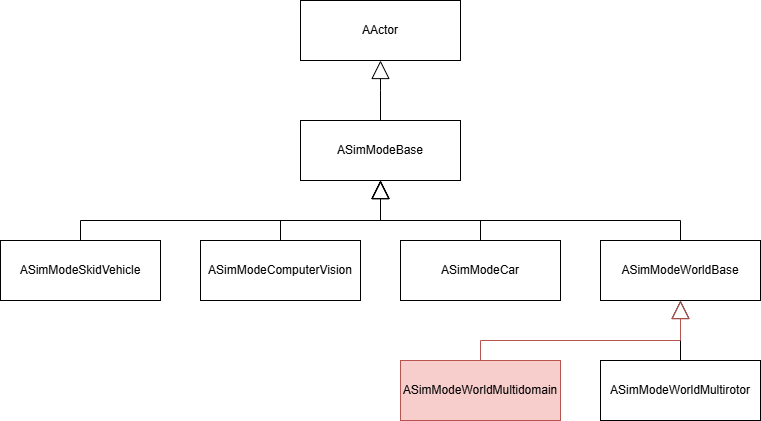
\includegraphics[width=0.7\textwidth]{graphics/simmode_hierarchy_extended.png}
    \caption{\small Modified UML Class Hierarchy for Cosys-AirSim Simulation Modes.}
    \label{fig:simmode_hierarchy_extended}
\end{figure}
\noindent
Table \ref{tab:simmode_modifications} provides a comprehensive summary of the modifications and additions implemented across the core files to support the multidomain simulation architecture.
\begin{longtable}{|p{0.22\textwidth}|p{0.28\textwidth}|p{0.42\textwidth}|}
    \caption{\small Summary of Modifications for Multidomain Simulation Modes.}
    \label{tab:simmode_modifications} \\
    \hline
    \textbf{Class} & \textbf{Method / Attribute} & \textbf{Modification Description} \\
    \hline
    \endfirsthead % This defines the header for the FIRST page
    
    \multicolumn{3}{c}{} \\
    \hline
    \textbf{Class} & \textbf{Method / Attribute} & \textbf{Modification Description} \\
    \hline
    \endhead % This defines the header for ALL SUBSEQUENT pages
    
    \hline
    \multicolumn{3}{r}{} \\
    \endfoot % This defines the footer for the bottom of the page when it breaks
    
    \hline
    \endlastfoot % This defines the footer for the very end of the table
    
    % --- AirSimSettings.hpp ---
    \texttt{\seqsplit{AirSimSettings}}
    & kSimModeTypeMultidomain
    & Creates a constant, file-specific pointer that points to the text `Multidomain'. \\ \cline{2-3}
    
    & \texttt{\seqsplit{loadCameraDirectorSetting}}
    & Defines the camera director follow distance (-8) and Z-position (-3) for Multidomain simulation mode. \\ \cline{2-3}
    
    & \texttt{\seqsplit{loadClockSettings}}
    & Sets clock type to \texttt{SteppableClock} unless a PX4 enabled vehicle is present (which triggers \texttt{ScalableClock}). \\ \cline{2-3}
    
    & \texttt{\seqsplit{createDefaultSensorSettings}}
    & Specifies default sensors (IMU, magnetometer, GPS, barometer) for Multidomain mode. \\ \cline{2-3}
    
    & \texttt{\seqsplit{loadCoreSimModeSettings}}
    & Enforces "FastPhysicsEngine" as the default physics engine if none is specified in settings. \\ \cline{2-3}
    
    & \texttt{\seqsplit{createDefaultVehicle}}
    & Generates a default drone and a default car if Multidomain mode is selected and no vehicles are specified. \\ 
    \hline
    
    % --- SimModeBase ---
    \texttt{\seqsplit{ASimModeBase}}
    & \texttt{createApiServer} 
    & Returns a dynamic array of smart pointers. \\ \cline{2-3}
    
    & \texttt{api\_servers\_} \newline (replacing \texttt{api\_server\_})
    & Refactored from a single smart pointer to multiple smart pointers holding multiple objects. \\ \cline{2-3}
    
    & \texttt{pawn\_to\_vehicle\_map} 
    & Added map data structure relating pawn pointers to their vehicle types. \\ \cline{2-3}

    & \texttt{addPawnToMap} 
    & Added method to insert entries into the tracking map. \\ \cline{2-3}
    
    & \texttt{getVehicleType} 
    & Added method returning the vehicle type string from the map (or an empty string if not found). \\
    \hline

    % --- SimModeWorldBase ---
    \texttt{\seqsplit{ASimModeWorldBase}}
    & \texttt{initializeForPlay} 
    & Established a bifurcated physics pipeline: drones use AirSim's \texttt{\seqsplit{PhysicsWorld}}, while cars use Unreal Engine's native physics. \\ \cline{2-3}

    & \texttt{registerPhysicsBody} 
    & Restricted custom physics registration to dynamically spawned drones, preserving the bifurcated architecture. \\ \cline{2-3}

    & \texttt{Tick} 
    & Separated state updates by physics domain to prevent thread conflicts between custom and native physics. \\ \cline{2-3}

    & \texttt{reset} 
    & Implemented independent resets for the custom physics world (drones) and Unreal Engine's native physics (cars). \\ 
    \hline

    % --- SimModeSkidVehicle ---
    \texttt{\seqsplit{ASimModeSkidVehicle}}
    & \texttt{createApiServer} 
    & Modified to return a dynamic array of smart pointers instead of a single smart pointer. \\ 
    \hline

    % --- SimModeWorldMultirotor ---
    \texttt{\seqsplit{ASimModeWorldMultirotor}} 
    & \texttt{createApiServer} 
    & Modified to return a dynamic array of smart pointers instead of a single smart pointer. \\ 
    \hline
    
    % --- SimModeComputerVision ---
    \texttt{\seqsplit{ASimModeComputerVision}}
    & \texttt{createApiServer} 
    & Modified to return a dynamic array of smart pointers instead of a single smart pointer. \\  \cline{2-3}
    
    & \texttt{\seqsplit{isPaused}} \& \texttt{\seqsplit{pause}}
    & Overridden to use Unreal's \texttt{\seqsplit{UGameplayStatics}} to safely check, stop, or resume simulation execution. \\ 
    \hline
    
    % --- SimModeCar ---
    \texttt{\seqsplit{ASimModeCar}}
    & \texttt{createApiServer} 
    & Modified to return a dynamic array of smart pointers instead of a single smart pointer. \\  \cline{2-3}
    
    & \texttt{\seqsplit{isPaused}} \& \texttt{\seqsplit{pause}} 
    & Overridden to use an internal variable (\texttt{\seqsplit{current\_clockspeed\_}}) to pause, or resume by scaling time in Unreal. \\ 
    \hline
    
    % --- SimModeWorldMultidomain ---
    \texttt{\seqsplit{ASimModeWorldMultidomain}} \newline (New Class)
    & \texttt{BeginPlay} \& \texttt{EndPlay} 
    & Initializes the physics world, and safely stops the physics engine before Unreal dismantles the world. \\ \cline{2-3}
    
    & \texttt{setupClockSpeed} 
    & Configures internal timing, dynamically scaling the physics control loop to allow time manipulation safely. \\ \cline{2-3}
    
    & \texttt{createApiServer} 
    & Opens two separate RPC servers simultaneously: port 41451 (Multirotors) and port 41452 (Cars). \\ \cline{2-3}
    
    & \texttt{getExistingVehiclePawns} 
    & Scans environment for drones and cars, pushing them to the internal tracking map with type flags. \\ \cline{2-3}
    
    & \texttt{isVehicleTypeSupported}
    & Whitelists \texttt{\seqsplit{kVehicleTypeSimpleFlight}} and \texttt{\seqsplit{kVehicleTypePhysXCar}}. \\ \cline{2-3}
    
    & \texttt{\seqsplit{getVehiclePawnPathName}}
    & Acts as a fallback for spawning default blueprints. \\ \cline{2-3}
    
    & \texttt{getVehiclePawnEvents} \newline \texttt{getVehiclePawnCameras} 
    & Retrieves specific event handlers and camera attachments for a given pawn. \\ \cline{2-3}
    
    & \texttt{initializeVehiclePawn} \newline \texttt{createVehicleSimApi} 
    & Triggers domain-specific initializations and instantiates core simulation APIs based on the vehicle domain. \\
    \hline

    % --- SimHUD ---
    \texttt{ASimHUD} 
    & \texttt{getSimModeFromUser} 
    & Added a message to the initial sequence dialogue prompting the user to choose a multidomain or monodomain simulation. \\ \cline{2-3}
    
    & \texttt{createSimMode} 
    & Spawns the \texttt{ASimModeWorldMultidomain} actor based on user choice or settings. \\ 
    \hline
    
\end{longtable}